\chapter{Estado del Arte}

En este capítulo hablaremos sobre la situación de la industria del entretenimiento digital hoy en día, qué es un \textit{roguelike}, los elementos que dificultan y facilitan el uso de diferentes programas y \textit{software} a ciertos sectores de la sociedad como invidentes o daltónicos, qué opciones de accesibilidad existen en diferentes sistemas operativos y las razones por las que hemos elegido ciertas de las características de las que queremos dotar a nuestro proyecto.

\section{La industria del entretenimiento digital en la actualidad}

Desde sus primeros pasos hasta hoy en día, tal y como sucede con muchas de las novedades en el mundo del entretenimiento y la cultura, el sector del ocio digital ha sufrido cierto estigma por una gran parte de la población, siendo censurado y degragado en mayor o menor medida, no tan solo por cierta parte de la sociedad, pero también por muchos medios de comunicación y gobiernos. A pesar de que hoy en día este problema todavía está activo\footnote{Es común que cada año en Australia se censuren algunos juegos como \href{http://goo.gl/hFrQah}{Paranautical Activity} por razones que otras formas de entretenimiento y cultura como películas o libros no se ven tan afectados.}, la industria se ha expandido tanto (consolas, PC, en el navegador, Facebook y móvil), que cada vez es más complicado encontrar a alguien que no haya jugado a algo en las últimas semanas y ya es algo que forma parte del día a día de mucha parte de la población.

\footnote{\href{http://www.statista.com/graphic/1/317604/video-games-industry-revenue-platform-germany.jpg}{La venta de videojuegos en Alemania crece año tras año, pero el mayor aumento de beneficio se está centrando en el mercado de los juegos para móvil}} 

Las ventas 

\section{\textit{Roguelikes.}}

\subsection{Qué es y orígenes}

En 1983, Michael Toy y Glenn Wichman crearon un videojuego llamado Rogue\footnote{Desde 2014 este juego se encuentra disponible en \href{https://archive.org/details/msdos_Rogue_1983}{archive.org}} que acabó defiendo un género.

Las características principales que definieron a Rogue y que, por extensión, definieron al género de los \textit{roguelikes} inicialmente, son:

\paragraph{Dificultad}: Rogue es un videojuego difícil que obligará al jugador a rejugarlo una y otra vez, intentando llegar más lejos que la anterior vez gracias a ir aprendiendo los funcionamientos del mismo.

\paragraph{Aleatoriedad}: Cada vez que el jugador comienza una partida nueva se encontrará con ciertos elementos que han cambiado con respecto a la anterior: el mapa es diferente, los elementos y enemigos se encuentran en sitios distintios, los propios objetos han cambiado... causando que cada partida tenga un grado de dificultad pseudo-aleatorio dependiendo de la semilla con la que estos elementos han sido generados.

\paragraph{Progresión}: Una de las frases más escuchadas en las críticas que Rogue recibió tras su lanzamiento es que el jugador sentía la necesidad de intentar llegar más lejos en cada ocasión\footnote{Jerry Pournelle habló de ello en \href{http://archive.org/stream/byte-magazine-1984-03/1984_03_BYTE_09-03_Simulation#page/n47/mode/2up}{este artículo}}. Esto viene dado, sobre todo, por la sensación de progresión y de que en cada \textit{run}\footnote{Palabra comúnmente usada en estos géneros y que se refiere a una partida desde su inicio hasta que el jugador pierde} el jugador va mejorando.  

\begin{figure}[h!]
		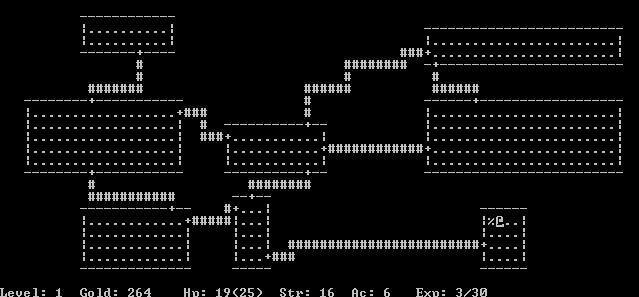
\includegraphics[width=\textwidth,height=\textheight,keepaspectratio]{C:/Users/Dario/Documents/GitHub/roomsgamedoc/img/roguegame.PNG}
	\caption{Screenshot de \href{https://en.wikipedia.org/wiki/File:Rogue_Unix_Screenshot_CAR.PNG}{dominio público} del videojuego Rogue}
	\label{fig:roguegame}
\end{figure}

\subsection{En la actualidad}

\subsection{Elementos \textit{roguelike} en nuestro proyecto}